\section{Криволинейные системы координат}

\subsection{Определение}

\begin{definition}
  Открытое связное множество называется \textit{областью}.
\end{definition}

\begin{definition}
  Отображение $f : D \subset \mathbb{R}^n \to G \subset \mathbb{R}^n$ называют
  \textit{гладким отображением класса $C^r(D)$} при
  $1 \leqslant r < \infty,~r = \infty$ или $r = \omega$, если оно
  дифференцируемо до порядка $r$ включительно, бесконечно дифференцируемо или
  аналитично соответственно.
\end{definition}

\begin{definition}
  \textit{Криволинейной системой координат} в области $D \subset \mathbb{R}^n$
  называют систему гладких функций $(x_1 (y_1, \dots, y_n), \dots,
  x_n (y_1, \dots, y_n))$, задающих взаимно однозначное отображение области $D$
  на некоторую область $G \subset \mathbb{R}^n$, причём якобиан
  \begin{equation}
    J(y) = \det
    \left(
    \begin{array}{ccc}
      \frac{\partial x_1}{\partial y_1}(y) & \dots &
        \frac{\partial x_n}{\partial y_1}(y) \\
      \vdots & \ddots & \vdots \\
      \frac{\partial x_1}{\partial y_n}(y) & \dots &
        \frac{\partial x_n}{\partial y_n}(y)
    \end{array}
    \right)
  \end{equation}
  отличен от нуля во всех точках области $D$.
\end{definition}

\begin{remark}
  Отличие от нуля якобиана $J(y)$ при всех $y \in D$ гарантирует, что обратное
  к $f(y)$ отображение $f^{-1}(x)$ также является гладким.
\end{remark}

\begin{definition}
  Взаимо однозначное и взаимно непрерывное отображение называется
  \textit{гомеоморфизмом}.
\end{definition}

Таким образом, криволинейная система координат задаётся двумя гладкими взаимно
однозначными отображениями $f(y)$ и $f^{-1}(x)$, устанавливающими гомеоморфизм
между множествами $D$ и $G$.

\begin{definition}
  Гладкий гомеоморфизм $f : D \to G$ класса $C^r(D)$ называют
  \textit{диффеоморфизмом класса $C^r(D)$}, а множества $D$ и $G$ называют
  \textit{диффеоморфными}.
\end{definition}

Итак, криволинейная система координат в области $D \subset \mathbb{R}^n$
является некоторым диффеоморфизмом $f : D \to G \subset \mathbb{R}^n$ с
ненулевым якобианом.

\subsection{Замена координат}

Пусть $y \in \mathbb{R}^n$, и в области $D \subset \mathbb{R}^n$ две системы
координат $x(y) = (x_1(y), \dots, x_n(y))$ и $z(y) = (z_1(y), \dots, z_n(y))$
заданы отображениями $f : D \to G_1 \subset \mathbb{R}^n$ и
$g : D \to G_2 \subset \mathbb{R}^n$.

\begin{definition}
  \textit{Заменой координат} $x$ на $z$ называется отображение
  $\psi : G_1 \to G_2$, задаваемое формулой $\psi = g \circ f^{-1}$.
\end{definition}

\begin{remark}
  Замена $\psi : G_1 \to G_2$ --- диффеоморфизм с ненулевым якобианом, то есть
  это криволинейная система координат в $G_1 \subset \mathbb{R}^n$.
\end{remark}

\begin{figure}[H]
  \centering
  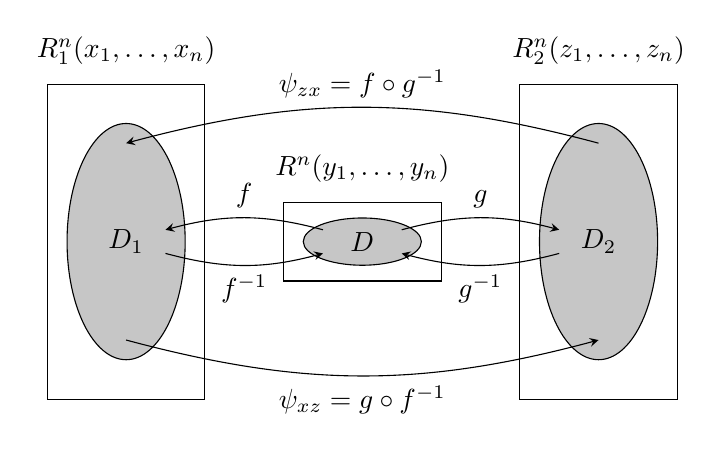
\begin{tikzpicture}
    \draw (0,0) rectangle (2,4);
    \draw (1,4) node[rectangle,
    label=above:{$\mathbb{R}_1^n(x_1,\dots,x_n)$}]{};

    \draw[fill=gray!45] (1,2) node[rectangle]{$D_1$}
    ellipse (0.75 and 1.5);

    \draw (3,1.5) rectangle (5,2.5);
    \draw (4,2.5) node[rectangle,
    label=above:{$\mathbb{R}^n(y_1,\dots,y_n)$}]{};

    \draw[fill=gray!45] (4,2) node[rectangle]{$D$}
    ellipse (0.75 and 0.3);

    \draw (6,0) rectangle (8,4);
    \draw (7,4) node[rectangle,
    label=above:{$\mathbb{R}_2^n(z_1,\dots,z_n)$}]{};

    \draw[fill=gray!45] (7,2) node[rectangle]{$D_2$}
    ellipse (0.75 and 1.5);

    \draw [stealth-,out=15,in=165] (1,3.25) to node[sloped,above]
    {$\psi_{zx} = f \circ g^{-1}$} (7,3.25);

    \draw [-stealth,out=-15,in=-165] (1,0.75) to node[sloped,below]
    {$\psi_{xz} = g \circ f^{-1}$} (7,0.75);

    \draw [stealth-,out=15,in=165] (1.5,2.15) to node[sloped,above]
    {$f$} (3.5,2.15);

    \draw [-stealth,out=-15,in=-165] (1.5,1.85) to node[sloped,below]
    {$f^{-1}$} (3.5,1.85);

    \draw [-stealth,out=15,in=165] (4.5,2.15) to node[sloped,above]
    {$g$} (6.5,2.15);

    \draw [stealth-,out=-15,in=-165] (4.5,1.85) to node[sloped,below]
    {$g^{-1}$} (6.5,1.85);
  \end{tikzpicture}

  \caption{}
  \label{fig:coords_map}
\end{figure}

\subsection{Список литературы}
\begin{enumerate}
  \item \cite{lectures}
\end{enumerate}

